\documentclass[11pt,a4paper]{article}
\usepackage[utf8]{inputenc}
\usepackage[english]{babel}
\usepackage{amsmath}
\usepackage{amsfonts}
\usepackage{amssymb}
\usepackage{graphicx}
\graphicspath{{../figures/}}
\author{Jacob Heden Malm}
\title{DD2424 Assignment 3}
\begin{document}
\maketitle

\section{Analytic gradient computations}

Since I wrote my code in python I could not use the provided ComputeGradsNum() method. Instead I performed a sanity check by attempting to over fit my network to a small amount of training examples and monitoring the development of the loss value. I wrote a method called sanity\_check() where I passed in 100 data points and attempted to get my loss values as low as possible. I did this by training on the entire batch of data passed in for 1000.\\

Here is an example of the development of the loss values through training on this very limited data set.

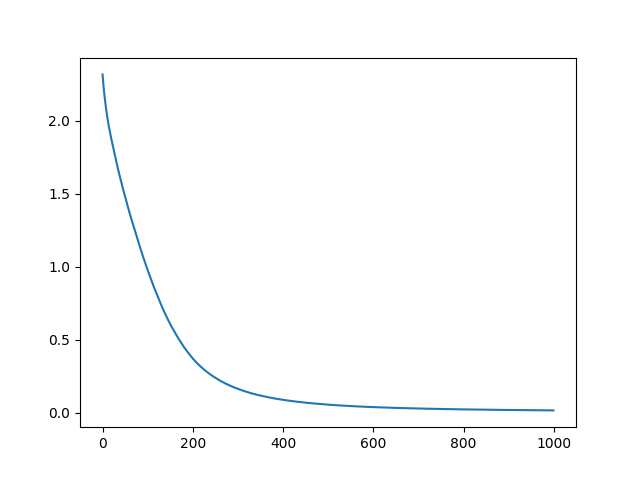
\includegraphics[width=\textwidth]{sanity_check.png}


The shape of the development of the loss function is almost exactly what we'd expect a nice satisfying 1/x curve. This suggests, since the derivative of this curve is logarithmic, that the rate of improvement decreases the more we have already learned, which makes sense. We also manage to get almost arbitrarily close to 0, suggesting that the network learns to recognize the training set perfectly, which allows us to conclude that the gradient computations are in fact working.

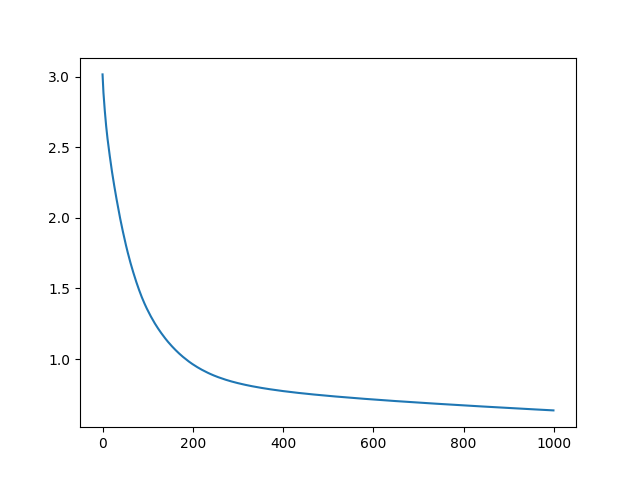
\includegraphics[width=\textwidth]{sanity_check_lambda-01.png}


When we set lambda to 0.01 we can see that we do not reach quite as low a value in our loss development, as expected, however we are still able to fit our net arbitrarily well.


\section{Training a k-layer network}

I began by training a 2 layer network with 1 hidden layer of 50 nodes. 
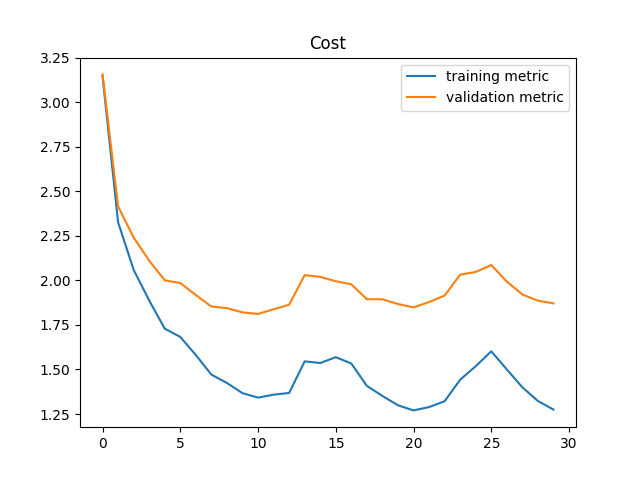
\includegraphics[width=\textwidth]{cost_k=1.png}
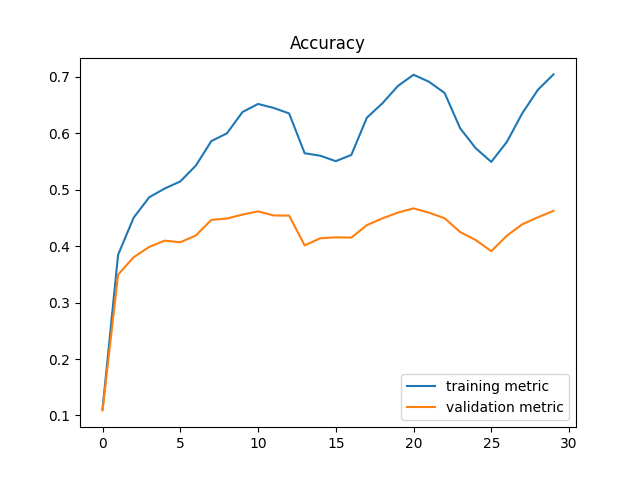
\includegraphics[width=\textwidth]{accuracy_k=1.png}\\

We can compare this with the results we got for a similar network from assignment 2\\
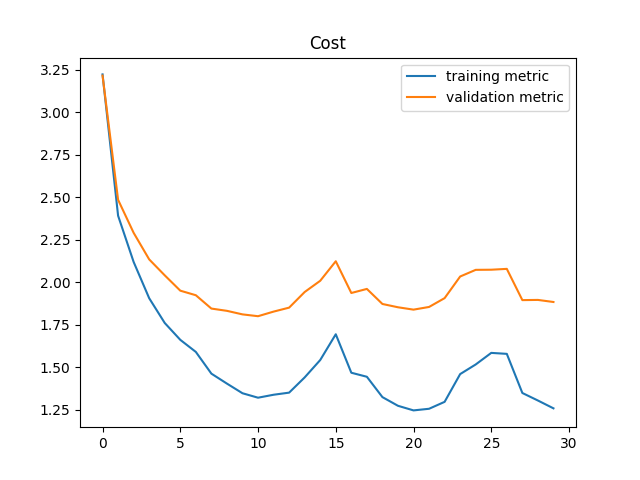
\includegraphics[width=\textwidth]{ns=800_cost.png}
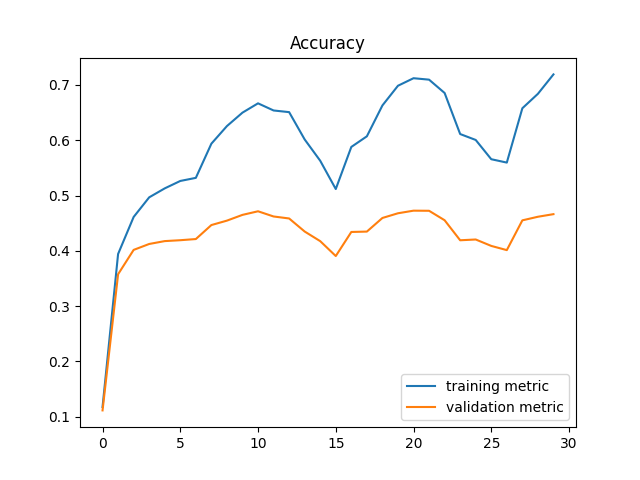
\includegraphics[width=\textwidth]{ns=800_accuracy.png}

The results look pretty similar.\\

If we add a second hidden layer also of 50 nodes, our metrics look as follows\\
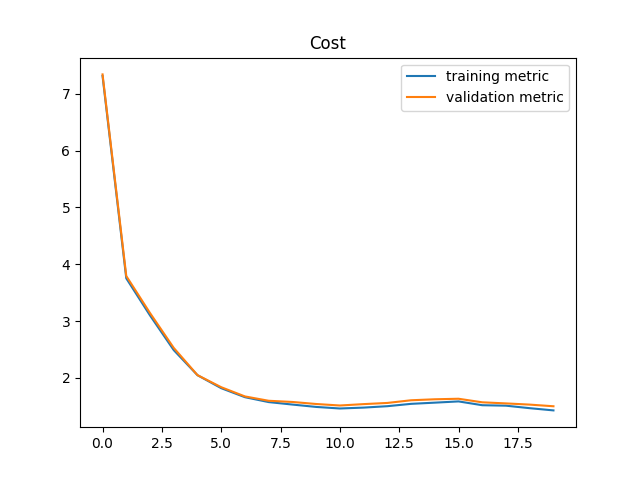
\includegraphics[width=\textwidth]{cost_k=2.png}
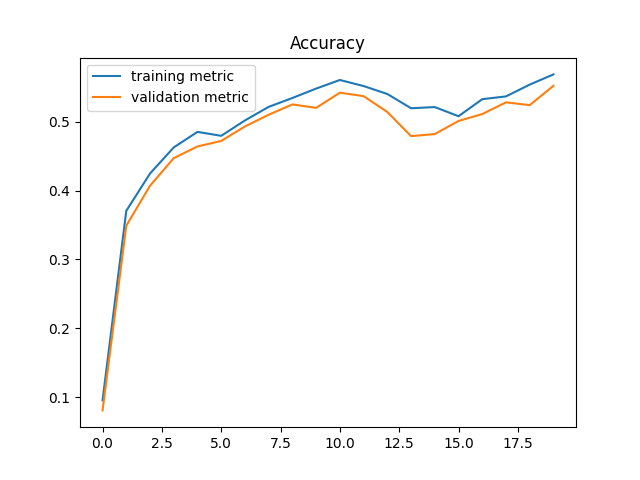
\includegraphics[width=\textwidth]{accuracy_k=2.png}
These graphs look pretty nice, the decrease in over fitting can be attributed to me switching to using the full training set.\\


The accuracy this 3 layer network exhibits on the test set is 0.5253333333333333. This test accuracy is however higher than my most performant network from assignment 2, suggesting that there's some value in increasing the depth of the network. If we investigate this assumption by attempting to train a 9 layer network, we see the following results\\


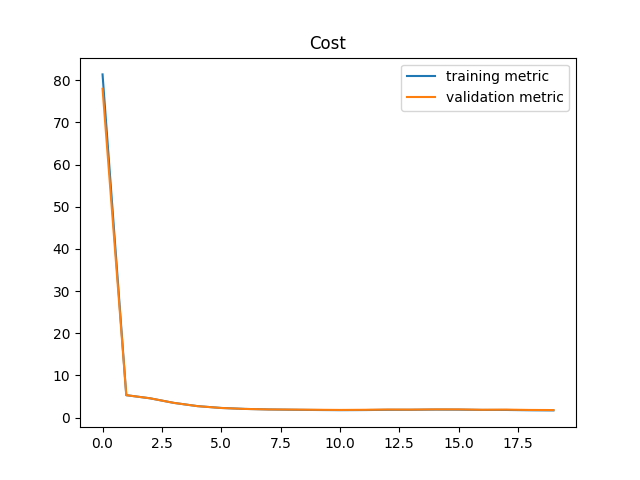
\includegraphics[width=\textwidth]{cost_k=9.png}
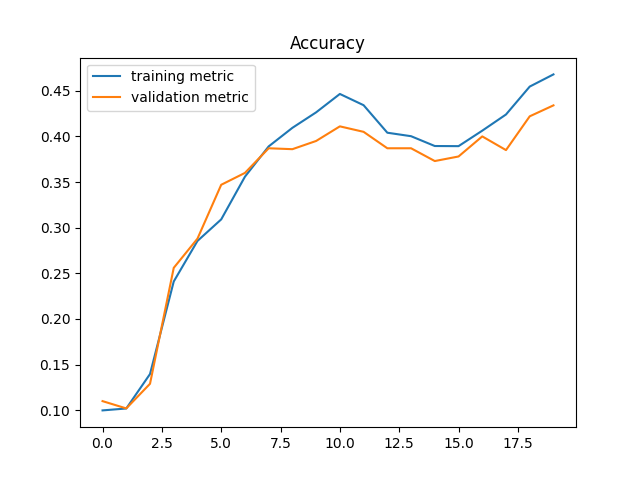
\includegraphics[width=\textwidth]{accuracy_k=9.png}

The test accuracy of this 9 layer network was 0.4488888888888889, almost an 8\% point decrease from our 3 layer network, no bueno.

\section{Implementing batch normalization}

I performed the same sanity check as before, but on a network with batch normalization.

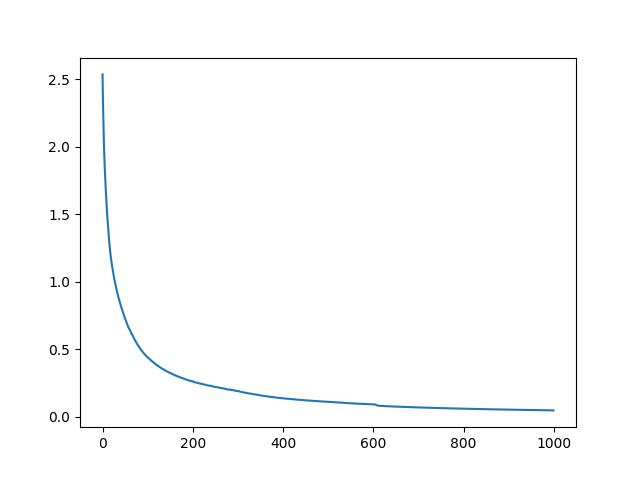
\includegraphics[width=\textwidth]{sanity_check_batch_norm.png}

We can see that the loss development looks the same as previously, suggesting that our gradient computations with batch normalization work well.

\section{Training a k-layer network with batch normalization}

Test accuracy on 2 layer network: 0.5173333333333333
Test accuracy on 3 layer network: 0.5361111111111111

\subsection{Search for optimal lambda value}

I began by performing a coarse search with 10 uniformly sampled lambda values from the range 1E-5, 1E-5. The validation accuracy is plotted here.

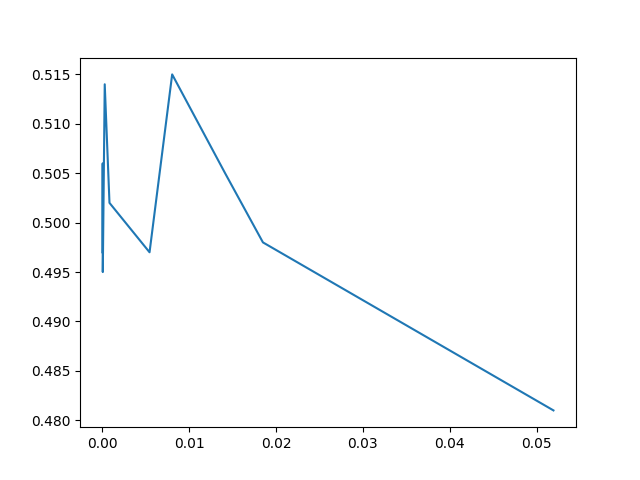
\includegraphics[width=\textwidth]{coarse_search.png}

As we can see the area of interest is roughly 0-0.015, with more emphasis to be placed on the upper end of this range.\\

Thus I performed a fine search by pulling 30 samples from a uniform distribution with domain [1E-4, 1E-2].


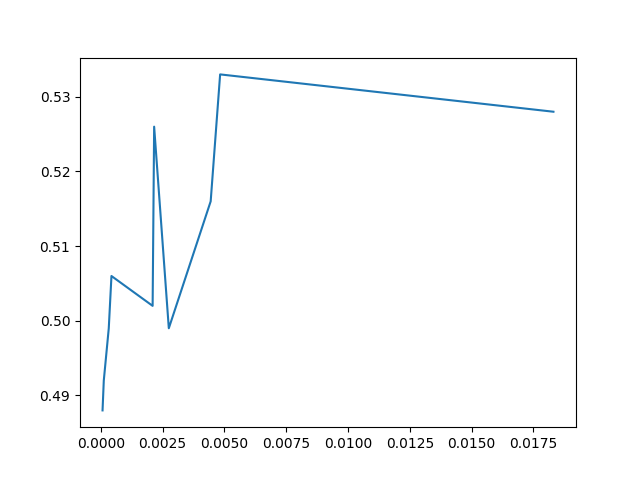
\includegraphics[width=\textwidth]{fine_search.png}


Test accuracy of 3 layer network with optimal lambda:


\end{document}
